% NB: use pdflatex to compile NOT pdftex.  Also make sure youngtab is
% there...

% converting eps graphics to pdf with ps2pdf generates way too much
% whitespace in the resulting pdf, so crop with pdfcrop
% cf. http://www.cora.nwra.com/~stockwel/rgspages/pdftips/pdftips.shtml




\documentclass[10pt,aspectratio=169,dvipsnames]{beamer}
\usetheme[color/block=transparent]{metropolis}

\usepackage[absolute,overlay]{textpos}
\usepackage{booktabs}
\usepackage[utf8]{inputenc}


\usepackage[scale=2]{ccicons}

\usepackage[official]{eurosym}


\usepackage{tikz}
\usetikzlibrary{arrows.meta}

\usepackage{xcolor}

\makeatletter
\def\mathcolor#1#{\@mathcolor{#1}}
\def\@mathcolor#1#2#3{%
  \protect\leavevmode
  \begingroup
    \color#1{#2}#3%
  \endgroup
}
\makeatother

%use this to add space between rows
\newcommand{\ra}[1]{\renewcommand{\arraystretch}{#1}}


\setbeamerfont{alerted text}{series=\bfseries}
\setbeamercolor{alerted text}{fg=Mahogany}
\setbeamercolor{background canvas}{bg=white}


\newcommand{\R}{\mathbb{R}}

\def\l{\lambda}
\def\m{\mu}
\def\d{\partial}
\def\cL{\mathcal{L}}
\def\co2{CO${}_2$}



% for sources http://tex.stackexchange.com/questions/48473/best-way-to-give-sources-of-images-used-in-a-beamer-presentation

\setbeamercolor{framesource}{fg=gray}
\setbeamerfont{framesource}{size=\tiny}


\newcommand{\source}[1]{\begin{textblock*}{5cm}(10.5cm,8.35cm)
    \begin{beamercolorbox}[ht=0.5cm,right]{framesource}
        \usebeamerfont{framesource}\usebeamercolor[fg]{framesource} Source: {#1}
    \end{beamercolorbox}
\end{textblock*}}

\usepackage{hyperref}


%\usepackage[pdftex]{graphicx}


\graphicspath{{graphics/}}

\DeclareGraphicsExtensions{.pdf,.jpeg,.png,.jpg}



\def\goat#1{{\scriptsize\color{green}{[#1]}}}


\newcommand{\ubar}[1]{\text{\b{$#1$}}}

\let\olditem\item
\renewcommand{\item}{%
\olditem\vspace{5pt}}

\title{Energy System Modelling\\ Summer Semester 2020, Lecture 15}
%\subtitle{---}
\author{
  {\bf Dr. Tom Brown}, \href{mailto:tom.brown@kit.edu}{tom.brown@kit.edu}, \url{https://nworbmot.org/}\\
  \emph{Karlsruhe Institute of Technology (KIT), Institute for Automation and Applied Informatics (IAI)}
}

\date{}


\titlegraphic{
  \vspace{0cm}
  \hspace{10cm}
    \includegraphics[trim=0 0cm 0 0cm,height=1.8cm,clip=true]{kit.png}

\vspace{5.1cm}

  {\footnotesize

  Unless otherwise stated, graphics and text are Copyright \copyright Tom Brown, 2020.
  Graphics and text for which no other attribution are given are licensed under a
  \href{https://creativecommons.org/licenses/by/4.0/}{Creative Commons
  Attribution 4.0 International Licence}. \ccby}
}

\begin{document}

\maketitle


\begin{frame}

  \frametitle{Table of Contents}
  \setbeamertemplate{section in toc}[sections numbered]
  \tableofcontents[hideallsubsections]
\end{frame}


\section{Introduction to Flow Allocation}



\begin{frame}{Who uses transmission lines?}

  Consider a single transmission line in a complicated meshed grid.

  Can we say which consumers and generators are using it at any time?

  \vspace{.3cm}

  \centering
  \includegraphics[width=8.5cm]{line-nodes}

  \source{\href{https://www.iit.comillas.edu/docs/IIT-02-100I.pdf}{Comillas EC report, 2002}}

\end{frame}



\begin{frame}{Who uses transmission lines?}

  Basic answer: \alert{no}. Electricity gets \alert{thoroughly mixed} in the grid; electrons do not carry markers that say `from nuclear plant A' or `from wind plant B'.

  \vspace{.3cm}

  \centering
  \includegraphics[width=8.5cm]{line-nodes}

  \source{\href{https://www.iit.comillas.edu/docs/IIT-02-100I.pdf}{Comillas EC report, 2002}}

\end{frame}






\begin{frame}{What is flow allocation?}

  \alert{Flow allocation} refers to algorithms that assign the flow of power in electricity network assets (e.g. lines and transformers) to particular users (e.g. generators and consumers).

  \vspace{.3cm}

  \centering
  \includegraphics[width=8.5cm]{line-nodes}

  \source{\href{https://www.iit.comillas.edu/docs/IIT-02-100I.pdf}{Comillas EC report, 2002}}

\end{frame}





\begin{frame}{Why flow allocation is non-trivial and non-unique}

  There is \alert{no unique} way to do flow allocation. There are
  \alert{ambiguities} both at network junctions and due to multiple
  paths through the network (i.e. closed cycles).

  \vspace{.5cm}

  \begin{columns}
    \column[c]{.5\textwidth}


    \centering
  %https://tex.stackexchange.com/questions/270543/draw-a-graph-in-latex-with-tikz
  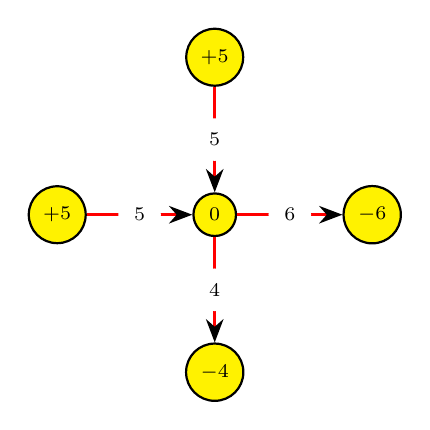
\begin{tikzpicture}
    \begin{scope}[every node/.style={circle,thick,draw,fill=yellow,font=\scriptsize}]
      \node (1) at (2,2) {$0$};
      \node (2) at (2,4) {$+5$};
      \node (3) at (0,2) {$+5$};
      \node (4) at (2,0) {$-4$};
      \node (5) at (4,2) {$-6$};
    \end{scope}

    \begin{scope}[>={Stealth[black]},
        every node/.style={fill=white,circle,font=\scriptsize},
        every edge/.style={draw=red,very thick,font=\scriptsize}]
      \path [->] (2) edge node {5} (1);
      \path [->] (3) edge node {5} (1);
      \path [->] (1) edge node {4} (4);
      \path [->] (1) edge node {6} (5);
    \end{scope}
  \end{tikzpicture}

\column[c]{.5\textwidth}


    \centering
  %https://tex.stackexchange.com/questions/270543/draw-a-graph-in-latex-with-tikz
  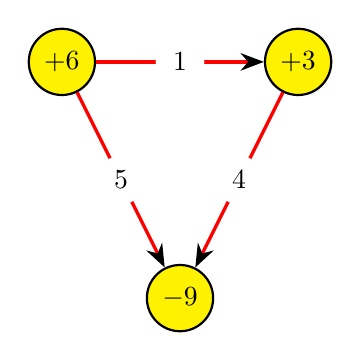
\begin{tikzpicture}
    \begin{scope}[every node/.style={circle,thick,draw,fill=yellow}]
      \node (1) at (3,3) {$+3$};
      \node (2) at (0,3) {$+6$};
      \node (3) at (1.5,0) {$-9$};
    \end{scope}

    \begin{scope}[>={Stealth[black]},
        every node/.style={fill=white,circle},
        every edge/.style={draw=red,very thick}]
      \path [->] (2) edge node {$1$} (1);
      \path [->] (2) edge node {$5$} (3);
      \path [->] (1) edge node {$4$} (3);
    \end{scope}
  \end{tikzpicture}

\end{columns}

\end{frame}




\begin{frame}{What is flow allocation?}

  Flow allocation gives a \alert{break-down} of the flow in each asset in terms of the network users.

  \vspace{.3cm}

  \centering
  \includegraphics[width=7.5cm]{marginal_participation_split_gen}

  \source{\href{https://doi.org/10.1049/iet-rpg.2014.0114}{Brown et al, IET, 2014}}

\end{frame}


\begin{frame}{What is flow allocation?}

  \alert{Different algorithms} deliver \alert{different results}, including:
  \begin{itemize}
  \item Assigning fractions of flow on each line to individual generators and consumers
  \item Assigning fractions of flow on each line to pairs of generators and consumers
  \item Matching consumers of power to generators of power via particular paths in the network
  \item Assigning fractions of flows to different groups, e.g. national vs. international, renewable vs. non-renewable
  \end{itemize}

  \vspace{.3cm}

  Some methods may not be suitable in certain circumstances, e.g. for
  HVDC lines or aggregated networks (principally because of cyclic
  flows).

\end{frame}




\begin{frame}{What is flow allocation useful for?}

  Flow allocation can be used to \alert{assign costs} to particular network actors of \dots
  \begin{itemize}
  \item operation and maintenance costs for existing network assets
  \item compensation for network losses
  \item new network assets
  \item grid connection charges for new generators
  \item redispatch
  \item international redispatch (multi-lateral remedial actions (MRAs))
  \end{itemize}

  \alert{Nota Bene}: Most of these use cases would \alert{not} be necessary in a
  market with \alert{nodal pricing} at (partial) \alert{equilibrium}. These use cases compensate for \alert{imperfect market design}.

  Flow allocation can also be used to increase understanding of the network,
  e.g. to increase public acceptance by seeing the source of network flows.

\end{frame}


\section{Algorithms for Flow Allocation}

\begin{frame}{What algorithms exist in the literature?}

  There are many algorithms for flow algorithms in literature, but \alert{no consensus} on best one.

  \begin{itemize}
    \item \alert{Flow tracing} (also called Bialek's method or Average Participation) assumes flow divides at junctions like water flow
    \item \alert{Marginal participation} uses the PTDF matrix to assess the flow sensitivity
    \item \alert{Aumann-Shapley} uses game theory for agents in the network
    \item \alert{With- and without transits} looks at domestic versus international transmission loading
    \item \alert{Virtual injection patterns} modifies flow tracing
  \end{itemize}

  We'll look at first two.

\end{frame}


\begin{frame}
  \frametitle{Flow tracing: Conservation of partial flows}
\begin{columns}[T]
  \begin{column}{7.5cm}
    \vspace{0.2cm}

    \alert{Power conservation} from KCL
    \begin{equation*}
      p_{n,t} = \sum_\ell K_{n,\ell} f_{\ell,t}
    \end{equation*}

    Separating \alert{in-flows} and \alert{out-flows},
    \begin{equation*}
      [p_{n}]_+ + \sum_m f_{m \to n} = [p_{n}]_- + \sum_m f_{n \to m}
    \end{equation*}

    \only<2>{
    allows to \alert{label} the energy entering the network and determine its mixing $q_{m,\alpha}$
    \begin{equation*}
      [p_{n,\alpha}]_+ + \sum_m q_{m,\alpha} f_{m \to n,t} = q_{n,\alpha}\left(  [p_{n,t}]_- + \sum_m f_{n \to m,t} \right)
    \end{equation*}

    Mixing is tracked all the way from sources to sinks.

    }
  \end{column}

  \begin{column}{6cm}
    \vspace{0.2cm}
    \only<1>{\includegraphics<1>[width=6cm]{flowtracing-example-flow.png}}
    \only<2>{\includegraphics<2>[width=6cm]{flowtracing-example-tracing.png}}

    \only<2>{
    \begin{equation*}
      \alpha \in \left\{ \mathcolor{blue}{blue}, \mathcolor{orange}{orange}, \mathcolor{red}{red} \right\}
    \end{equation*}
    }
  \end{column}
\end{columns}

\source{Jonas Hörsch}
\end{frame}


\begin{frame}
  \frametitle{Flow tracing: Synthetic 118-bus demonstration case}

  Electrical transmission grid model with a \alert{topology from IEEE
    118-bus} test case embedded into a figurative country bordered by
  an \alert{eastern coast for offshore wind} and equipped with
  \alert{conventional and renewable generators and loads}.

  \begin{figure}
    \makebox[-.5em][l]{\includegraphics[width=.7\linewidth]{map}}
    \includegraphics[width=.7\linewidth]{generation-caps-by-region}
  \end{figure}

  \source{\href{https://arxiv.org/abs/1609.02977}{Hörsch et al, 2017}}
\end{frame}



\begin{frame}
  \frametitle{Flow tracing: Usage of individual transmission lines}

  \begin{figure}
    \makebox[-.5em][l]{\includegraphics[width=.8\linewidth]{map}}
    \includegraphics[width=.8\linewidth]{transmission-caps-by-generation-and-link}
  \end{figure}

  \source{\href{https://arxiv.org/abs/1609.02977}{Hörsch et al, 2017}}
\end{frame}


\begin{frame}
  \frametitle{Marginal participation: Use the PTDF matrix}

  The Power Transfer Distribution Factor (PTDF) gives a linear relationship for the linear power flow between the nodal power injections $p_i$ and the flows $f_\ell$
  \begin{equation*}
    f_\ell =  \sum_i \textrm{PTDF}_{\ell i} p_i
  \end{equation*}

  This is already basically what we want - a \alert{sensitivity} of the flow in line $\ell$ to the power injection at node $i$.

  But remember that the PTDF \alert{depends strongly on the slack node}, related to a freedom to add a constant $c_\ell$, $ \textrm{PTDF}_{\ell i} \to      \textrm{PTDF}_{\ell i} + c_\ell $. This has \alert{no effect} on the flow:
  \begin{equation*}
     f_\ell =  \sum_i \textrm{PTDF}_{\ell i} p_i \to  \sum_i (\textrm{PTDF}_{\ell i} + c_\ell) p_i = \sum_i \textrm{PTDF}_{\ell i} p_i + c_\ell \sum_i p_i =  \sum_i \textrm{PTDF}_{\ell i} p_i
  \end{equation*}

  We can use this freedom to choose the $c_\ell$ such that there is an equal contribution of net consumers and net generators to each line.

\end{frame}


\begin{frame}
  \frametitle{Marginal participation: Application to high-renewable European power system}

  Top graph: power generation in Europe over 8 simulated days.

  Bottom: total line loading in TWkm in the European system - offshore wind dominates.


  \centering
  \includegraphics[width=12cm]{stacked-gen-loading.pdf}

  \source{\href{https://doi.org/10.1049/iet-rpg.2014.0114}{Brown, 2014}}
\end{frame}



\begin{frame}
  \frametitle{Marginal participation: Application to high-renewable European power system}

  \begin{columns}[T]
  \begin{column}{7cm}

  Wind travels on average further than other energy sources, particularly in the case of offshore wind.

  \vspace{.5cm}

  \includegraphics[width=7cm]{distance-travelled.pdf}
  \end{column}
  \begin{column}{7cm}

    The share of electricity flowing outside domestic borders also increases as countries share renewable resources.

  \vspace{.5cm}

    \includegraphics[width=7cm]{stacked-domestic-foreign.pdf}
  \end{column}

  \end{columns}
  \source{\href{https://doi.org/10.1049/iet-rpg.2014.0114}{Brown, 2014}}

\end{frame}



\section{Practical Applications of Flow Allocation}

\begin{frame}{Where is flow allocation currently used?}

  Commission Regulation (EU) No 838/2010 sets the terms for inter-TSO compensation (ITC) in Europe for costs incurred by
  cross-border flows (`transits') for
  \begin{itemize}
  \item \alert{infrastructure usage} (total compensation limited to 100
    million~\euro/a until new metholodogy can be implemented; distributed today using
    transit-load factor `postage stamp' method)
  \item \alert{losses} (total compensation was 153 million~\euro{} in 2015 (losses valued at around 50~\euro/MWh),  assessed using With and Without Transit (WWT) method)
  \end{itemize}

  Flow allocation is also used around the world for cost allocation,
  e.g. in South America, the United States and Great Britain (where it's used for
  the G- and L-components of Transport Network Use of System (TNUoS)). German TSOs also examining using flow allocation for
  MRA cost-sharing.

  %http://www.acer.europa.eu/Official_documents/Acts_of_the_Agency/Publication/ITC%20Monitoring%20Report%202016.pdf

  %Losses: valued around 50 EUR/MWh

  %Not all countries agree on method to evaluate the losses

  % the losses related fee is calculated by dividing the WWT (With and Without Transit) Fund size by the sum of  scheduled import and export flows, net import and net export flows; and
\end{frame}



\begin{frame}{Application example in Europe: Flow tracing}

  For example the Bialek \alert{flow tracing method} (also called Average
  Participation (AP)) is like a ``water flow'' and stays relatively
  \alert{localised}:

  \vspace{.3cm}

  \centering
  \includegraphics[width=9cm]{AP-ES-FR}

    \source{\href{https://ec.europa.eu/energy/sites/ener/files/documents/2006_03_tso_compensation_mechanism.pdf}{CONSENTEC, Frontier EC report, 2006}}

\end{frame}




\begin{frame}{Application example in Europe: Marginal participation}

  Whereas the \alert{power-flow-sensitivity method} (also called Marginal Participation (MP))
  sees effects from nodes \alert{across the network}:

  \vspace{.3cm}

  \centering
  \includegraphics[width=9cm]{MP-ES-FR}

    \source{\href{https://ec.europa.eu/energy/sites/ener/files/documents/2006_03_tso_compensation_mechanism.pdf}{CONSENTEC, Frontier EC report, 2006}}

\end{frame}


\begin{frame}{Why flow allocation is non-trivial and non-unique}

  This results in \alert{very different} assessments of the amount of
  compensation due to each European country for \alert{transit flows} from
  other countries (AP versus MP for 2003):

  \centering
  \includegraphics[width=10cm]{MP-AP-2013}

    \source{\href{https://ec.europa.eu/energy/sites/ener/files/documents/2006_03_tso_compensation_mechanism.pdf}{CONSENTEC, Frontier EC report, 2006}}
\end{frame}



\begin{frame}{Why flow allocation is non-trivial and non-unique}

  They are also \alert{unstable} from year to year (example of MP for 2003 and 2004):


  \centering
  \includegraphics[width=11cm]{MP-2013-2014}

    \source{\href{https://ec.europa.eu/energy/sites/ener/files/documents/2006_03_tso_compensation_mechanism.pdf}{CONSENTEC, Frontier EC report, 2006}}
\end{frame}



\begin{frame}{Why flow allocation is non-trivial and non-unique}


  Therefore it is \alert{no wonder} that in the 7 years since
  Commission Regulation (EU) No 838/2010, there has been \alert{no
    agreement} on a new methodology for inter-TSO compensation.

  \vspace{1cm}

  Private quotation from Midcontinent Independent System Operator (MISO) employee: \\ ``Flow
  allocation is the \alert{single most contentious subject} I've ever
  encountered''.

  \vspace{1cm}


  We are looking at economics-based flow allocation, based on \alert{benefit to each user of line}.


  %\source{\href{https://ec.europa.eu/energy/sites/ener/files/documents/2003_11_cbt.pdf}{Comillas EC report, 2003}}
\end{frame}


\end{document}
